\section{Background and Related Works}
\label{sec:background}
%UPPRESSO is designed to be compatible with OpenID Connect (OIDC) and provide privacy protections based on the discrete logarithm problem. Next,

We introduce %OIDC \cite{OpenIDConnect}, to describe
  typical SSO login flows,
 and discuss existing privacy-preserving solutions and other related works.

\subsection{OpenID Connect and SSO Services}
\label{subsec:OIDC}
OIDC is one of the most popular SSO protocols. % for web applications. %As other SSO protocols \cite{SAMLIdentifier}, OIDC
%It involves three entities, i.e., {\em users}, the {\em identity provider (IdP)}, and {\em relying parties (RPs)}.
Users and RPs initially register at the IdP with their identities %($ID_U$, $ID_{RP}$ and $PID_U$ in some schemes) %(or $PID_{RP}$ in some schemes)
and other necessary information such as user credentials %(i.e., passwords or key pairs)
 and RP endpoints (i.e., the URLs to receive identity tokens).
% below can be removed
%The IdP should maintain these attributes securely.

%\vspace{1mm}
%\noindent\textbf{Implicit Login Flow.}
OIDC supports three types of login flows: implicit flow, authorization code flow, and hybrid flow (i.e., a mix-up of the other two).
%In the implicit flow, an {\em id token} is generated as the identity token, which contains a user identifier, an RP identifier, the issuer (i.e., IdP), the validity period, and other requested attributes. The IdP signs the id token using its private key to ensure integrity, and sends it to the RP through the user.
%In the authorization code flow, the IdP binds an authorization code with the RP, and sends it to the RP through the user; then, the RP establishes an HTTPS connection to the IdP and uses the authorization code with the RP's credential to obtain the user's identifier and other attributes.
%UPPRESSO is compatible with all three flows.
They work with different steps to request and receive identity tokens,
    but with the common security requirements of identity tokens.
We introduce the implicit flow and present our designs based on this flow.
Section \ref{sec:discussion} discusses the supports of authorization code flows.

\begin{figure}[t]
  \centering
  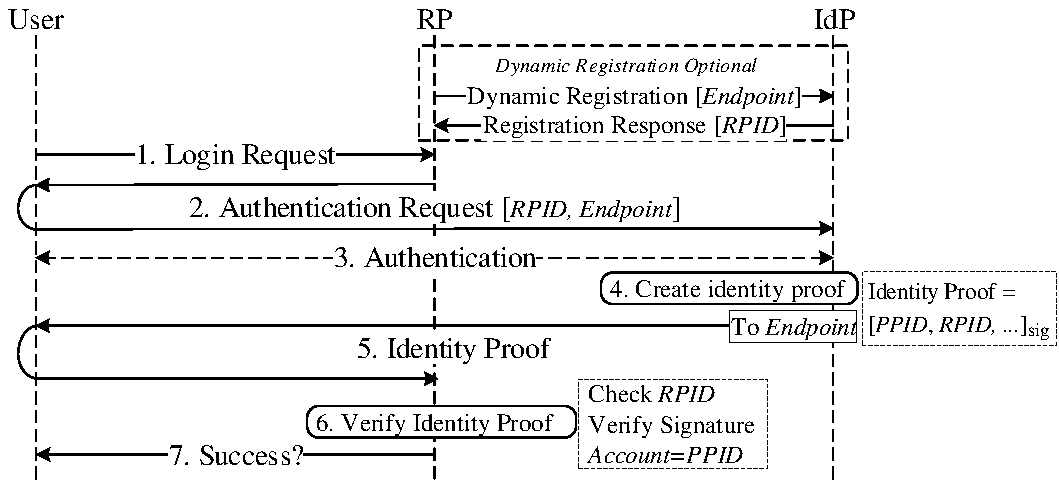
\includegraphics[width=0.9\linewidth]{fig/OIDC1.pdf}
  \caption{The implicit SSO login flow of OIDC.}
  \label{fig:OpenID}
%  \vspace{-5mm}
\end{figure}

As shown in Figure \ref{fig:OpenID}, a user firstly initiates a login request to an RP.
Then, the RP constructs an identity-token request with its own identity
 and the scope of requested user attributes.
This request is redirected to the IdP.
After authenticating the user,
    the IdP issues an identity token
        which is forwarded by the user to the RP endpoint.
The token contains a user identity (or pseudo-identity),
    the RP identity, a validity period, the requested user attributes, etc.
Finally, the RP verifies the received identity token and
 allows the user to login as the  enclosed (pseudo-)identity.
The user's operations including redirection, authorization, and forwarding,
    are implemented in a software called user agent (i.e., a browser).

%Before issuing the identity token,
%    the IdP obtains the user's authorization to enclose the requested attributes.
 %   which are maintained at the IdP by the user.
%The IdP is also a web service.
%The identity token is usually signed by the IdP,
%    and transmitted through secure channels such as TLS/HTTPS.

%extracts user's identifier and returns the authentication result to the user (Step 7).


\begin{table*}[tb]
\footnotesize
    \caption{Privacy-Preserving Solutions of SSO and Identity Federation.}
    \centering
    \begin{tabular}{|c|c|c|c|c|c|c|}
  \hline
  \multirow{3}*{\textbf{~~Solution~~}} &
  \multicolumn{3}{c|}{\textbf{SSO Feature} - supported $\CIRCLE$, unsupported $\Circle$, or partially $\LEFTcircle$} & \multicolumn{3}{c|}{\textbf{Privacy Threat} - prevented $\CIRCLE$ or not $\Circle$} \\ \cline{2-7}
  & User Identity & User Authentication & IdP-Confirmed Selective  & IdP-based & RP-based & Collusive Attack \\
  & at an RP & Only to the IdP &  Attribute Provision & Login Tracing & Identity Linkage & by the IdP and RPs \\\hline\hline
  OIDC with PPID \cite{NIST2017draft} & $\CIRCLE$ & $\CIRCLE$ & $\CIRCLE$ & $\Circle$ & $\CIRCLE$ & - \\ \hline
  BrowserID \cite{BrowserID} & $\CIRCLE$ & $\LEFTcircle$$^1$ & $\Circle$ & $\CIRCLE$ & $\Circle$ & - \\ \hline
  SPRESSO \cite{SPRESSO} & $\CIRCLE$ & $\CIRCLE$ & $\Circle$$^2$ & $\CIRCLE$ & $\Circle$ & - \\ \hline
  PRIMA \cite{prima} & $\CIRCLE$ & $\Circle$ & $\CIRCLE$ & $\CIRCLE$ & $\Circle$ & - \\ \hline
  PseudoID \cite{PseudoID} & $\CIRCLE$ & $\Circle$ & $\Circle$$^3$ & $\CIRCLE$ & $\CIRCLE$ & $\CIRCLE$ \\ \hline
  EL PASSO \cite{ELPASSO} & $\CIRCLE$ & $\Circle$ & $\CIRCLE$ & $\CIRCLE$ & $\CIRCLE$ & $\CIRCLE$ \\ \hline
  UnlimitID \cite{UnlimitID} & $\CIRCLE$ & $\Circle$ & $\CIRCLE$ & $\CIRCLE$ & $\CIRCLE$ & $\CIRCLE$ \\ \hline
  Opaak \cite{Opaak} & $\LEFTcircle$$^4$ & $\Circle$ & $\Circle$ & $\CIRCLE$ & $\CIRCLE$ & $\CIRCLE$ \\ \hline
  Fabric Idemix \cite{hyperledge-idemix} & $\Circle$$^5$ & $\Circle$ & $\CIRCLE$ & $\CIRCLE$ & $\CIRCLE$ & $\CIRCLE$ \\ \hline
  U-Prove \cite{uprov} & $\CIRCLE$ & $\Circle$ & $\LEFTcircle$$^6$ & $\CIRCLE$ & $\CIRCLE$ & $\CIRCLE$ \\ \hline
  UPPRESSO & $\CIRCLE$ & $\CIRCLE$ & $\CIRCLE$ & $\CIRCLE$ & $\CIRCLE$ & $\Circle$ \\ \hline
\end{tabular}
    \label{tbl:comparison-protocol}
\flushleft
{\footnotesize
1. A BrowserID user generates an \emph{ephemeral} private key to sign every ``subsidiary'' token,
 which is verified by the RP.\\
2. SPRESSO can be extended to provide user attributes in then tokens, while the prototype does not support it.\\
3. Blindly-signed user attributes can be selectively provided using zero-knowledge proofs,
    but not implemented in the prototype \cite{PseudoID}.\\
4. Opaak supports exclusive pseudonym options: (\emph{a}) linkable within an RP but unlinkable across multiple RPs and (\emph{b}) unlinkability for any two actions.\\
5. In the original design of Idemix \cite{idemix}, every user logins to an RP with a unique account.\\
6. A U-Prove token may contain some attributes \emph{invisible} to the IdP, in addition the ones confirmed by the IdP.}
\end{table*}


The following features are supported in widely-used popular SSO solutions \cite{NIST2017draft,OpenIDConnect,rfc6749,SAML,SAMLIdentifier}.
\\\textbf{User Identity at an RP.}
The identity tokens facilitate the target RP to identify each user as a unique account at this RP,
    and this account links the user's multiple login instances to this RP
        for customized services.
%On the contrary, in anonymous SSO systems \cite{WangWS13,HanCSTW18,HanCSTWW20}
%        the RP only verifies whether he is a legitimate user authenticated by the IdP
%            and receives no information to distinguish every user.
\\\textbf{User Authentication Only to the IdP.}
A ``pure'' SSO protocol  \cite{OpenIDConnect,rfc6749,SAML} does not include authentication steps:
    the authentication between a user and the IdP is conducted independently.
This
    enables the IdP to authenticate users by any appropriate means (e.g., password,
one-time password, and multi-factor authentication).
It eliminates the authentication steps between users and an RP,
        and RPs only verify tokens issued by the IdP.
A user holds only the credential to authenticate himself to the IdP,
    and the burden is greatly reduced.
If this credential was lost or leaked,
    the user only renews it at the IdP.
However, if a user proves some non-ephemeral secret to RPs and this secret is valid across multiple login instances
    (i.e., authentication steps are actually involved),
                the user has to notify each RP if it was leaked. %during its validity period. %(or even the user logins from another computer).
\\\textbf{IdP-Confirmed Selective Attribute Provision.}
The IdP usually provides user attributes in the tokens \cite{OpenIDConnect,rfc6749,SAML},
    in addition to user (pseudo-)identities.
These attributes are maintained by users at the IdP.
%    for example,
%        when Facebook provides social networking services,
%         it also issues identity tokens enclosing user identities and various attributes.
Before enclosing attributes in a token,
    the IdP obtains the user's authorization;
    or the provided attributes are selected by the user.
So no distinctive attributes such as telephone number, Email address, etc.,
        are enclosed in the identity tokens of privacy-preserving SSO systems.

%\vspace{1mm}
%\noindent\textbf{RP Dynamic Registration.}
%In addition to manual registrations,
%    OIDC also supports dynamic registrations
%    for an RP to register by online means \cite{DynamicRegistration}.
%The (unregistered) RP sends a registration request
%        with endpoints to receive identity tokens (and other information),
%        to the IdP.
%After a successful registration,
% the IdP assigns a unique RP identity in the response.
%

%UPPRESSO leverages this function and slightly modifies the dynamic registration process to implement the {\em $PID_{RP}$ registration} process (see details in Section \ref{sec:UPPRESSO}.C), which allows an RP to generate different privacy-preserving RP identifiers and register them with the IdP.


\subsection{Privacy-Preserving SSO and Identity Federation}
\label{subsec-solutions}
Table \ref{tbl:comparison-protocol} lists privacy-preserving solutions of SSO and identity federation.
Widely-used SSO protocols \cite{OpenIDConnect,rfc6749,SAML,SAMLIdentifier} allow a user to login to RPs,
%    after being authenticated by the IdP,
        without by himself holding any permanent secret verified by RPs
        or maintain accounts for these RPs.
While keeping this user convenience,
 existing privacy-preserving SSO \cite{BrowserID,SPRESSO,NIST2017draft} prevents the IdP-based login tracing or the RP-based identity linkage,
    and UPPRESSO prevents both of them.

On the contrary, identity federation enables a user registered at the IdP to be accepted by other parties,
            with different accounts sometimes,
        but more user operations are involved than those of SSO.
Privacy-preserving identity federation \cite{ELPASSO,UnlimitID,hyperledge-idemix,PseudoID,Opaak}
    protects privacy against even collusive attacks by the IdP and the RPs,
    but requires a user to (\emph{a}) hold long-term secrets verified by RPs,
            in addition to the authentication credentials for the IdP,
                and (\emph{b}) manage the accounts at different RPs by himself.
That is, there are actually some authentication steps between the user and RPs (or called asynchronous authentication \cite{ELPASSO}).


Pairwise pseudonymous identifiers (PPIDs) are recommended \cite{NIST2017draft}
 and specified in SSO protocols \cite{OpenIDConnect, SAMLIdentifier} to protect user privacy against curious RPs.
When issuing an identity token,
        the IdP encloses a user PPID (but not the identity at the IdP).
Given a user,
    the IdP assigns a unique PPID based on the target RP,
    so collusive RPs cannot link the users.
PPIDs cannot prevent the IdP-based login tracing,
 for the IdP needs the RP identity to issue tokens.



Some solutions prevent the IdP-based login tracing,
    but vulnerable to the RP-based identity linkage.
In BrowserID \cite{BrowserID} (formerly known as Firefox Accounts \cite{FirefoxAccount} and Mozilla Persona \cite{persona}),
 the IdP %(called the primary identity authority in BrowserID)
  issues a special token (called user certificate) to bind a user identity to an \emph{ephemeral} public key,
 so the user utilizes the private key to sign a ``subsidiary'' token (called identity assertion)
    to bind the target RP's identity and sends both tokens to the RP.
The PRIMA IdP signs a credential binding a verification key and a set of user attributes \cite{prima}, and the key is viewed as the user identity.
The user selectively provides IdP-confirmed attributes to an RP using his signing key \cite{Oblivion}. % cooperatively with the IdP.
In SPRESSO \cite{SPRESSO} an RP assigns a verifiable one-time pseudo-identity to itself in each login instance.
Then, the IdP generates an identity token binding this RP pseudo-identity. %and the user identity.
In these schemes \cite{BrowserID,prima,SPRESSO}
    collusive RPs could link a user based on his unique identity in the tokens (or credentials).


PseudoID \cite{PseudoID} introduces an independent token service in addition to the IdP,
    to  \emph{blindly} sign an access token binding a pseudonym and a user secret.
The user unblinds this token,
 and the IdP will assert it,
    which allows the user to login to an RP using his secret.
Two kinds of privacy threats are prevented, because (\emph{a}) the RP's identity is not enclosed in the access token
    and (\emph{b}) the user encloses different pseudonyms when visiting RPs.
Collusive attacks by the IdP and RPs are also prevented,
    for they cannot link two blindly-signed tokens.

% the user must use the secret to login to RP, because no RP identity is enclosed in the token.


%However, the user has to permanently keep the secret preimage for each account in an RP.

In EL PASSO \cite{ELPASSO}, after authenticating a user,
    the IdP signs an anonymous credential \cite{anon-credential} binding a secret,
         both of which are kept on the user's device.
When attempting to login to an RP,
    the user proves that he is the owner of this credential without exposing the secret,
        and discloses selective attributes in the credential.
Although one credential is proved to multiple RPs,
        user-maintained pseudonyms and anonymous credentials prevent the RPs, even when collusive with the IdP, from linking the users across the RPs.
UnlimitID \cite{UnlimitID} presents similar designs based on anonymous credentials \cite{anon-credential},
        to prevent collusive attacks by the IdP and RPs.
NEXTLEAP \cite{nextleap} adopts UnlimitID for anonymous secure messaging.

%    but a user has to by himself manage pseudonyms for different RPs.
%For example,
%    the RP domain (e.g., \verb+www.RP.com+) is used as a factor to locally generate the user's account (or pseudonym) at this RP.

Anonymous credentials \cite{anon-credential-2001,anon-credential} are utilized in flexible ways.
Opaak \cite{Opaak} keeps IdP-signed anonymous credentials in mobile phones as pseudonym tokens,
    which bind a user's secret key.
The Idemix anonymous credential system \cite{idemix}
 is integrated in Hyperledger Fabric \cite{hyperledge-idemix} to implement completely-unlinkable pseudonyms
        and IdP-confirmed selective attribute disclosure.
After a user retrieves a U-Prove token \cite{uprov,uprove-conference} from the IdP,
    it enables the user to authenticate himself and selectively disclose attributes to an RP.

